\section{Analysis of Results}

\subsection{Accuracy of Tracking}

When it worked, \underline{Lucas-Kanade Affine} seemed most accurate:
\begin{figure}[H]
  \centering
  \begin{minipage}{.45\textwidth}
    \centering
    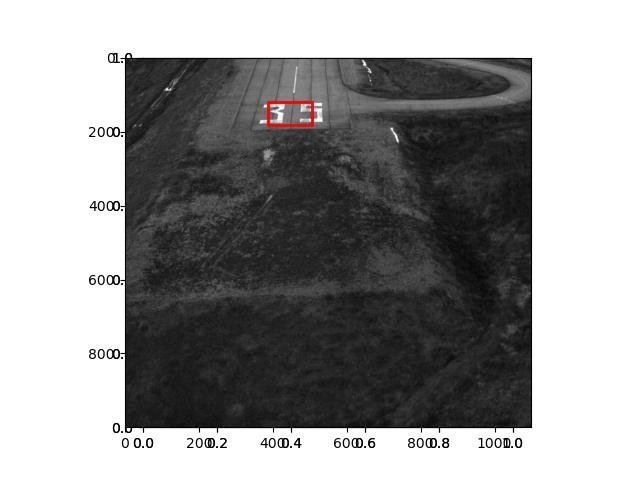
\includegraphics[width=\textwidth]{./figures/lk/landing/frame000040.jpg}
    \caption{LK, Frame $40$}
  \end{minipage}
  \begin{minipage}{.45\textwidth}
    \centering
    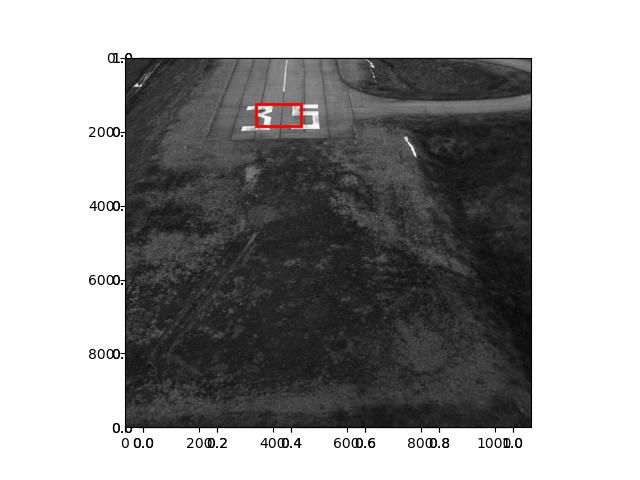
\includegraphics[width=\textwidth]{./figures/lk/landing/frame000049.jpg}
    \caption{LK, Frame $49$}
  \end{minipage}
  \begin{minipage}{.45\textwidth}
    \centering
    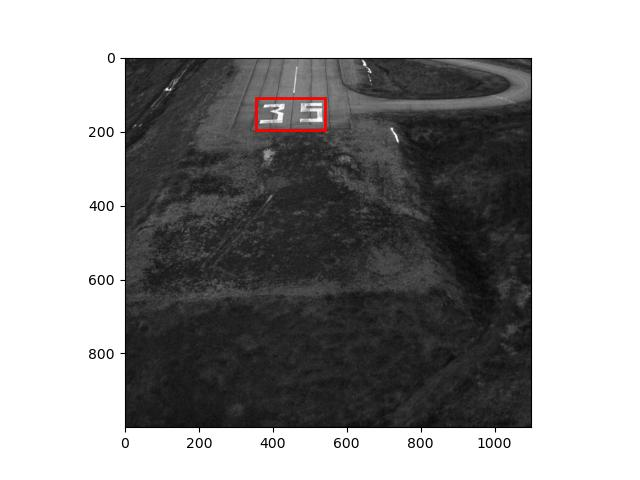
\includegraphics[width=\textwidth]{./figures/lk_affine/landing/frame000040.jpg}
    \caption{LK Affine, Frame $40$}
  \end{minipage}
  \begin{minipage}{.45\textwidth}
    \centering
    \includegraphics[width=\textwidth]{./figures/lk_affine/landing/frame000049.jpg}
    \caption{LK Affine, Frame $49$}
  \end{minipage}
  \begin{minipage}{.45\textwidth}
    \centering
    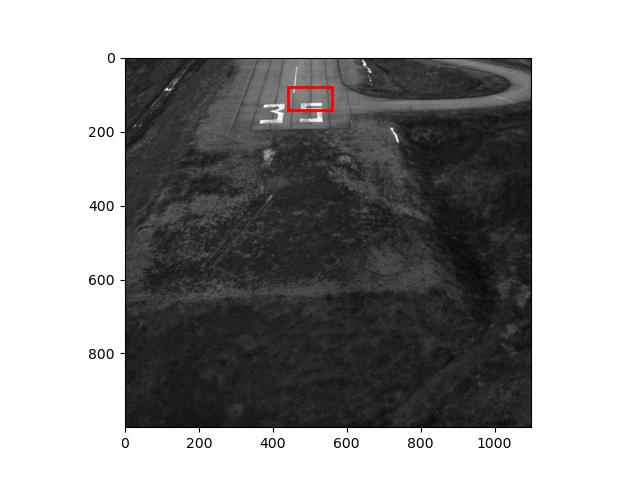
\includegraphics[width=\textwidth]{./figures/ic_affine/landing/frame000040.jpg}
    \caption{IC Affine, Frame $40$}
  \end{minipage}
  \begin{minipage}{.45\textwidth}
    \centering
    \includegraphics[width=\textwidth]{./figures/ic_affine/landing/frame000049.jpg}
    \caption{IC Affine, Frame $49$}
  \end{minipage}
\end{figure}

\subsection{Robustness of Tracking}

Both of the affine transformations (Lucas-Kanade affine and Inverse-Compositional Affine)
were thrown off in the third video and seemed to stick to one of the street lights
as the car moved.
Here's the exact place where that happens in Lucas-Kanade
(same place for Inverse-Compositional Affine, but not shown here):

\begin{figure}[H]
  \centering
  % minipage
  \begin{minipage}{.45\textwidth}
    \centering
    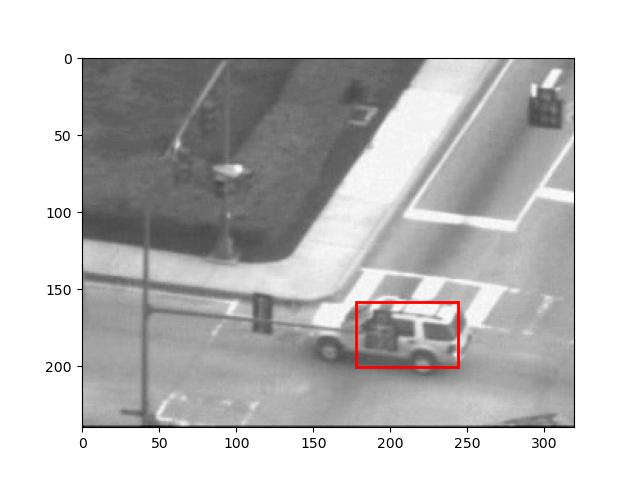
\includegraphics[width=.8\textwidth]{./figures/lk_affine/car2/frame000125.jpg}
    \caption{Frame $125$}
  \end{minipage}
  \hfill
  % minipage
  \begin{minipage}{.45\textwidth}
    \centering
    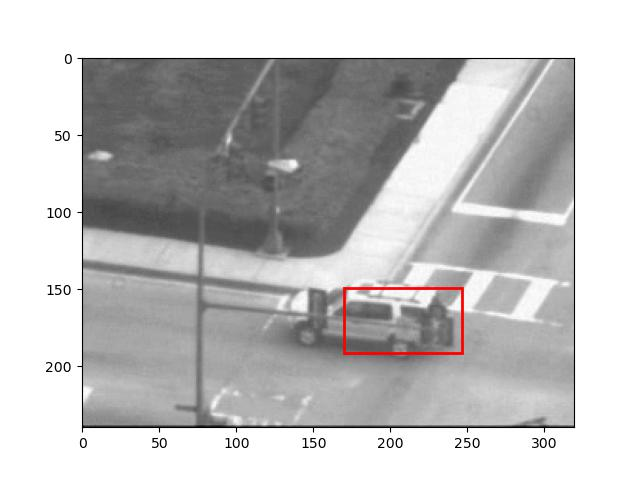
\includegraphics[width=.8\textwidth]{./figures/lk_affine/car2/frame000135.jpg}
    \caption{Frame $135$}
  \end{minipage}
  \hfill
  % minipage
  \begin{minipage}{.45\textwidth}
    \centering
    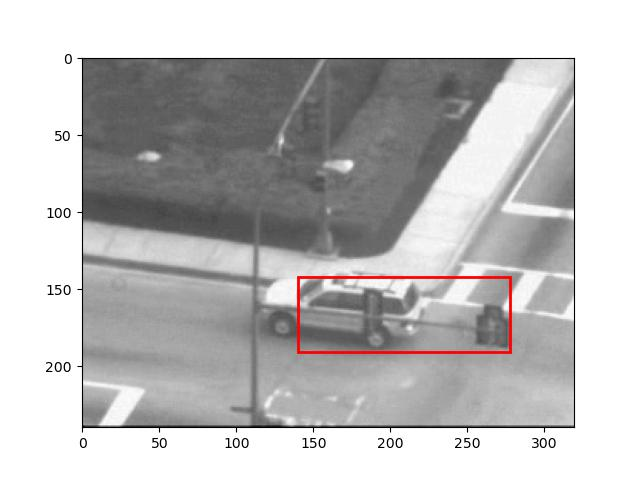
\includegraphics[width=.8\textwidth]{./figures/lk_affine/car2/frame000145.jpg}
    \caption{Frame $145$}
  \end{minipage}
  % minipage
  \begin{minipage}{.45\textwidth}
    \centering
    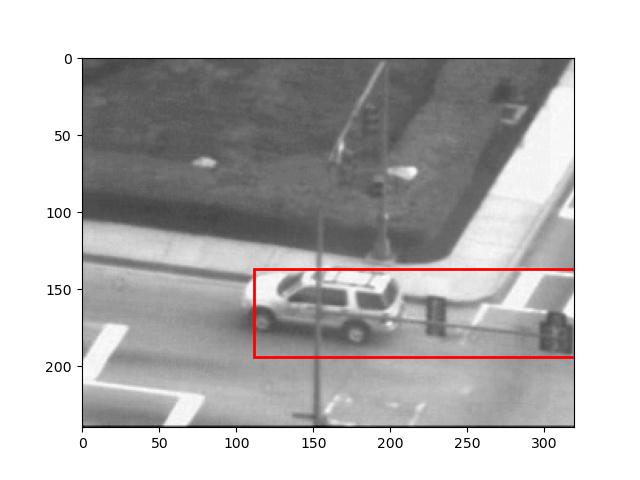
\includegraphics[width=.8\textwidth]{./figures/lk_affine/car2/frame000155.jpg}
    \caption{Frame $155$}
  \end{minipage}
  % minipage
  \begin{minipage}{.45\textwidth}
    \centering
    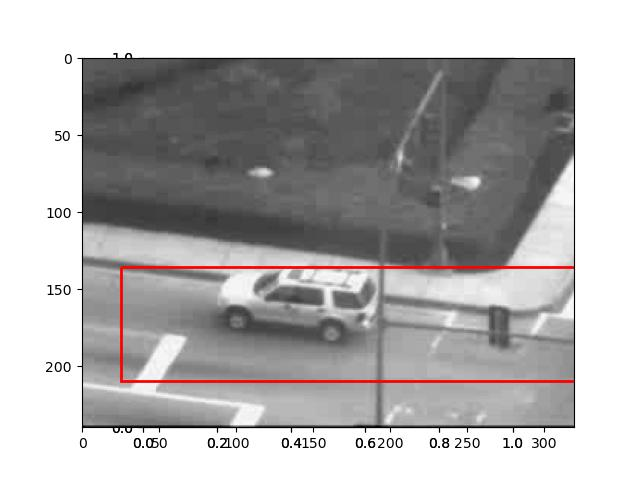
\includegraphics[width=.8\textwidth]{./figures/lk_affine/car2/frame000165.jpg}
    \caption{Frame $165$}
  \end{minipage}
  % minipage
  \begin{minipage}{.45\textwidth}
    \centering
    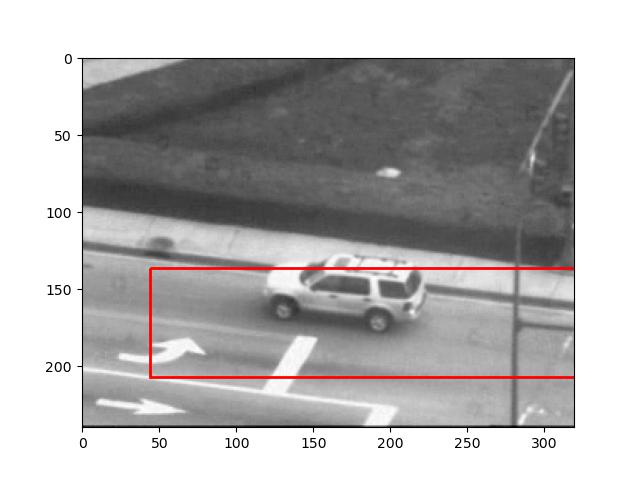
\includegraphics[width=.8\textwidth]{./figures/lk_affine/car2/frame000175.jpg}
    \caption{Frame $175$}
  \end{minipage}
\end{figure}

This suggests that the Lucas-Kanade affine and Inverse-Compositional affine optical flow
algorithms might be more sensitive to changes in the scene than the Lucas-Kanade transformation.
